\chapter{Introduction}
\section{The group}
The group consisted of six students from Computer Science at NTNU, each possessing different technical skills, but all were third year students in the Informatics Bachelor programme.

\begin{description}
	\item{Jeppe Eriksen}\hfill \\
		Experience with Java, MySQL, and basic Android development.
	\item{Bjørn Arve Fossum}\hfill \\
		Experience with Java, MySQL, PHP and C\#.
	\item{Ståle Semb Hauknes}\hfill \\
		Experience with Java, MySQL, PHP and Arduino$\texttrademark$.
	\item{Wilhelm Walberg Schive}\hfill \\
		Experience with Java, MySQL, and knew the basics of Arduino$\texttrademark$ project development.
	\item{Nina Margrethe Smørsgård}\hfill \\
		Experience with Java, MySQL, \LaTeX, and basics Android development.
	\item{Robin Tordly}\hfill \\
		Experience with Java, Android, MySQL, PHP and SQLite.
\end{description}

\section{Problem description}
The project task was to develop a platform for easy use, setup and sharing of Physical User Interfaces (PUIs) for Arduino$\texttrademark$. The task was divided in three main parts: a market application, over the air installation and example PUIs.\\
\newline
The purpose of the market application was to allow users of Arduino$\texttrademark$ to browse and download PUI applications for their Arduino$\texttrademark$ board on a mobile Android device. This market app was to be a simplified version of e.g. Google Play, where users easily can browse and install whatever applications they desire. An application selected for installation in the market application should be prepared on the mobile device, and installed over the air on an Arduino$\texttrademark$ board using Bluetooth$\textsuperscript{\textregistered}$ . The example PUIs were mostly intended to demonstrate the feasibility of the finished product.

\section{The goal}
The goal of the project task was to make Arduino$\texttrademark$ easier to use for ordinary people, by allowing easy browsing, sharing and installation of applications on Arduino$\texttrademark$ boards. By developing an application for over the air installation of applications, the finished product should ease the process of both installing and updating PUIs on an Arduino$\texttrademark$.


\section{Definitions}
This is a list of terms and abbreviations used throughout the project report in order to clarify and explain their meaning.

\begin{description}

\item[Android:]\hfill \\
An operating system for mobile devices based on the Linux operating system. It is developed by Google and the Open Handset Alliance. Applications for Android devices are written in Java, and all the software is open source released under the Apache License.

\item[Apache:] \hfill \\
A software foundation focused on open source and community driven software.

\item[Arduino$\texttrademark$:]\hfill \\
A tool for making Physical User Interfaces (PUIs). It is an open-source physical computing platform based on a simple microcontroller board.

\item[AVRDude:]\hfill \\
This is a tool to upload programs to microcontrollers from the Unix command line. This software has a lot of features, such as reading and writing to the microcontroller's memory over a serial connection. This software can also compile your C code into an Intel Hex file, a file full of binary information, that can be sent to the Arduino$\texttrademark$ with the STK500 protocol. Normally this is done with a cable between a computer and the microcontroller.

\item[STK500:]\hfill \\
This is a standard protocol used by many microcontrollers to upload and download memory, including the Arduino$\texttrademark$.

\item[PUI:]\hfill \\
An acronym for Physical User Interface. A PUI is a user interface which interacts with digital information through the physical environment.

\end{description}

\section{Work breakdown structure (WBS)}
The WBS is a view on what work packages the project encompasses. It helps with communicating the work and processes to easily execute the project. The duration-time show how much estimated time one task requires, and gives an assessment on how much effort should be considered.\\
\newline
\textbf{The Dictionary View} is an organized table view of the WBS with a simple structure. The Duration column is an extension of the original Dictionary View.\\

\begin{longtable}{|m{0.1 \textwidth}|m{0.1 \textwidth}|m{0.2 \textwidth}|m{0.35\textwidth}|m{0.15 \textwidth}|}
\hline
	\rowcolor{Gray}
	\textbf{Level} & \textbf{WBS{ }Code} & \textbf{Element name} & \textbf{Definition} & \textbf{Duration}\\
	\endfirsthead% 
	\multicolumn{5}{l}%
	{{\bfseries Continued from previous page}} \\ \hline
	\rowcolor{Gray}
	\textbf{Level} & \textbf{WBS{ }Code} & \textbf{Element name} & \textbf{Definition} & \textbf{Duration}\\
\hline
	\endhead%
	\hline
 
	\hline \multicolumn{5}{|l|}{{Continued on next page}} \\ \hline
	\endfoot%
 
	\endlastfoot%

	1 & 1 & $\mu$C Software Store & All work to implement an application store for Arduinos and over the air innstallation with two example PUIs & \\
\hline
	2 & 1.1 & Project management & The work to initiate the project and distribute responsibilities & \\
\hline
	3 & 1.1.1 & Meetings with customer & Determine the project status and decide on requirements & \\
	 & 1.1.2 & Demonstration and play for the customer of the team's understanding of the requirements & Project team evaluates and proposes recommendations & \\
\hline
	 & 1.1.3 & Risk management & Creating risk analysis and agreements within the group and the project & \\
\hline
	 & 1.1.4 & Status report & Write the status report & \\
\hline
	2 & 1.2 & Planning & & \\
\hline
	3 & 1.2.1 & Requirements specification & & \\
\hline
	 & 1.2.2 & Determine Project team & Give each menber a role and distribute tasks & \\
\hline
	 & 1.2.3 & Supervisor meeting & Meeting wih supervisor for instruction and guidance & \\
\hline
	 & 1.2.4 & Develop project plan and use cases & & \\
\hline
	 & 1.2.5 & Research & & \\
\hline
	 & 1.2.5.1 & Research on over the air innstallation & Do research on bluetooth installation on arduinos & \\
\hline
	 & 1.2.5.2 & Research UbiCollab libraries & & \\
\hline
	2 & 1.3 & Execution & Programming and execution of the project & \\
\hline
	3 & 1.3.1 & Project kickoff meeting & First meeting with customer to evaluate knowledge and agree on further meetings & \\
\hline
	 & 1.3.2 & Verify \& validate user requirements & Determine whether the group is in tune with the customers vision of the project requirements & \\
\hline
	 & 1.3.3 & Design system & & \\
\hline	  
	 & 1.3.4 & & & \\
\hline
	 & 1.3.5 & Produce Software & & \\
\hline
	 & 1.3.6 & Instalation over the air implementation & & \\
\hline
	 & 1.3.7 & Documentation & & \\
\hline
	2 & 1.4 & Testing & & \\
\hline
	3 & 1.4.1 & Develop unit tests & & \\
\hline
	 & 1.4.2 & User testing & & \\
\hline
	 & 1.4.3 & Stress testing & & \\
\hline
	 & 1.4.4 & System Testing & & \\
\hline
	2 & 1.5 & Closeout & & \\
\hline
	3 & 1.5.1 & Creating final project report & & \\
\hline
	 & 1.5.2 & Delivery to customer & & \\
\hline
\end{longtable}
\captionof{table}{Work Breakdown Structure}


\textbf{The Tree Structure}, which is the most popular WBS format, presents an easy to understand view into the WBS. The Tree Structure is not easy to make and is created with a tool: Microsoft Word and SmartArt graphics.\\

\begin{figure}[H]
\vspace*{-1.5in}
\hspace*{-1.2in}
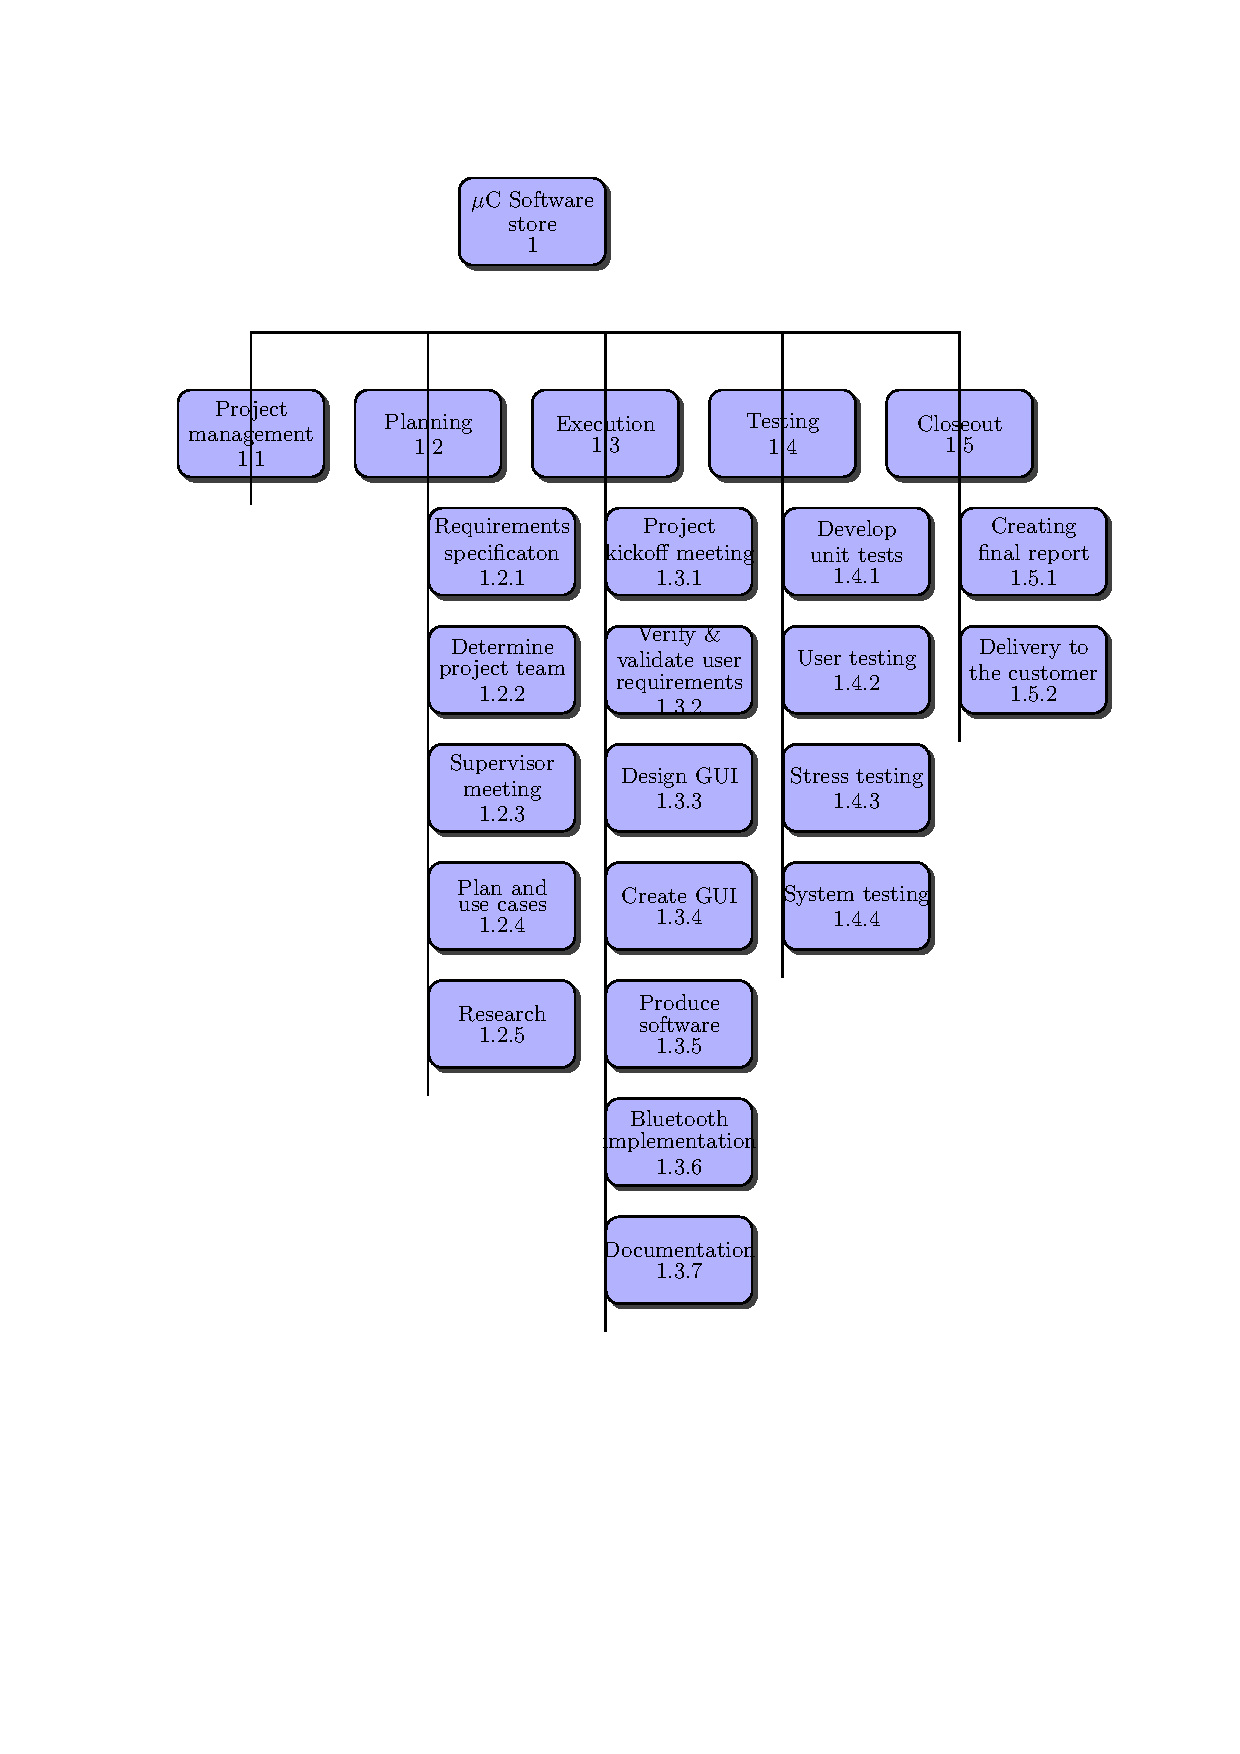
\includegraphics[trim=0cm 4cm 0cm 0cm]{figures/wbs-tree.pdf}
\captionof{figure}{WBS Tree}
\end{figure}
